\documentclass{article}
\usepackage[margin=1in]{geometry}
\usepackage{amsmath,amsthm,amssymb}
\usepackage{bbm,enumerate,mathtools}
\usepackage{tikz,pgfplots}
\usepackage{chessboard}
\usepackage[hidelinks]{hyperref}
\usepackage{multicol} % Problem 35

\newenvironment{question}{\begin{trivlist}\item[\textbf{Question.}]}{\end{trivlist}}
\newenvironment{note}{\begin{trivlist}\item[\textbf{Note.}]}{\end{trivlist}}
\newenvironment{references}{\begin{trivlist}\item[\textbf{References.}]}{\end{trivlist}}
\newenvironment{related}{\begin{trivlist}\item[\textbf{Related.}]\end{trivlist}\begin{enumerate}}{\end{enumerate}}


\begin{document}
\rating{3}{3}
Say that a \textit{minimally interpolable permutation} $f$ is a permutation of
$\{1, 2, \hdots, n\}$ such that no $k + 2$ of the
points $\{(1, f(1)),\hdots,(n, f(n))\}$ fall on a degree $k$ polynomial.
\begin{figure}[!h]
  \centering
  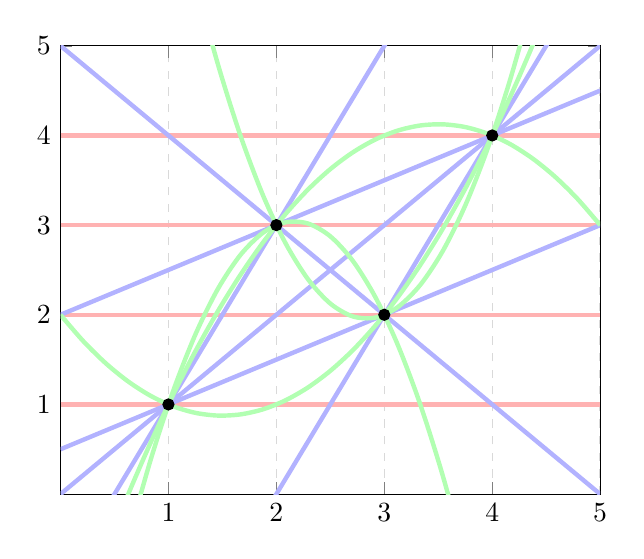
\begin{tikzpicture}[scale=1]
    \begin{axis}[
      xmin=0, xmax=5,
      ymin=0, ymax=5,
      domain=0:5,
      grid=both,
      grid style={line width=0.5pt, draw=gray!30, dashed},
      ytick={1,...,7},
      xtick={1,...,7},
      smooth
    ]
      \addplot[red!30, ultra thick] (x,1);
      \addplot[red!30, ultra thick] (x,2);
      \addplot[red!30, ultra thick] (x,3);
      \addplot[red!30, ultra thick] (x,4);

      \addplot[blue!30, ultra thick] (x,2*x-1);

      \addplot[blue!30, ultra thick] (x,x/2+1/2);
      \addplot[blue!30, ultra thick] (x,-x+5);

      \addplot[blue!30, ultra thick] (x,x);
      \addplot[blue!30, ultra thick] (x,2 + x/2);
      \addplot[blue!30, ultra thick] (x,-4 + 2*x);

      \addplot[green!30, ultra thick] (x,-3*x^2/2 + 13*x/2 - 4);
      \addplot[green!30, ultra thick] (x,-x^2/2 + 7*x/2 - 2);
      \addplot[green!30, ultra thick] (x,x^2/2 - 3*x/2 + 2);
      \addplot[green!30, ultra thick] (x,3*x^2/2 - 17*x/2 + 14);


      \addplot[mark=*] coordinates {(1,1)};
      \addplot[mark=*] coordinates {(2,3)};
      \addplot[mark=*] coordinates {(3,2)};
      \addplot[mark=*] coordinates {(4,4)};
    \end{axis}
  \end{tikzpicture}
  \caption{
    A minimally interpolable permutation of $\{1, 2, 3, 4\}$.
    (Degree 0 polynomials are plotted in red, degree 1 in blue, and degree 2 in green.)
  }
\end{figure}

\begin{question}
  Do such permutations always exist? If not, what is the least $N$ such that
  there is  a minimally interpolable function from $[n]$ into $[N]$?
\end{question}

\begin{related}
  \item How many minimally interpolable permutations exist?
  \item Does the number of minimally interpolable permutations increase as a
    function of $n$?
  \item Is there a method to explicitly construct a minimally interpolable
    permuation?
  \item If such permutations do not always exist, what is the least $M$ such
    that there exists a subset $S \subset [M]$ and a surjection
    $g\colon S\rightarrow [N]$ with the aforementioned property?
\end{related}
\begin{references}
  \item Problem 19.
  \item \url{https://oeis.org/A301802}
  \item \url{https://codegolf.stackexchange.com/q/160382/53884}
\end{references}
\end{document}
